%******************************************************************************
% KOMA-Script article scrartcl
%******************************************************************************
\documentclass[11.5pt, b5paper]{article} 

% Add here all the packages that will be used in the document
%******************************************************************************
% Packages 
%******************************************************************************
% For hyperlinks 
\usepackage{url}

% Add no chapters to the article 
\usepackage[nochapters]{classicthesis}

% Setup the page geometry
\usepackage{geometry}
\geometry{a4paper, total={210mm, 297mm}, 
left=20mm, right=20mm, top=20mm, bottom=20mm}

% Use tikz to add watermarks to the document
\usepackage{blindtext,tikz}
\usetikzlibrary{calc}

% Use the classicthesis style for the style of the document
\usepackage[nochapters]{classicthesis} 

% Use the currvita style for the layout of the document
\usepackage[LabelsAligned]{currvita} 

% Required for adding links	and customizing them
\usepackage{hyperref} 

 % Set link colors
\hypersetup{colorlinks, breaklinks, urlcolor=Maroon, linkcolor=Maroon}


% Add a list of new commands 
%******************************************************************************
% Commands 
%******************************************************************************
\newcommand{\latex}{\LaTeX\xspace}
\newcommand{\tex}{\TeX\xspace}

\usepackage{listings}
\usepackage{color}
\usepackage{graphicx}
\usepackage{caption}
\usepackage{subcaption}

\graphicspath{{images/report4/}}

\definecolor{dkgreen}{rgb}{0,0.6,0}
\definecolor{gray}{rgb}{0.5,0.5,0.5}
\definecolor{mauve}{rgb}{0.58,0,0.82}

\lstset{frame=tb,
  language=Java,
  aboveskip=3mm,
  belowskip=3mm,
  showstringspaces=false,
  columns=flexible,
  basicstyle={\small\ttfamily},
  numbers=none,
  numberstyle=\tiny\color{gray},
  keywordstyle=\color{blue},
  commentstyle=\color{dkgreen},
  stringstyle=\color{mauve},
  breaklines=true,
  breakatwhitespace=true,
  tabsize=3
}

%******************************************************************************
% DOCUMENT STARTS HERE 
%******************************************************************************
\begin{document}

% TITLE 
\title{\rmfamily\normalfont\spacedallcaps{
Report \#{4}
}}

% PROJECT NAME -> ADD YOUR PROJECT NAME HERE
\author{{\small Automatic Mandible Segmentation Using VTK}}

% AUTOMATIC DATE -> DON'T CHANGE MANUALLY
\date{\footnotesize{\today}}

% MAKE THE TITLE -> DON'T CHANGE MANUALLY
\maketitle

% DON'T INCLUDE THE ABSTRACT FOR THE MOMENT
% % \begin{abstract}
% \noindent Abstract
% \end{abstract}
 
%******************************************************************************
% TABLE OF CONTENTS (uncomment to show / comment to hide)
%******************************************************************************     
% \tableofcontents


%******************************************************************************
% Report Content
%******************************************************************************
\section{Report Details}
\begin{center}
\begin{tabular}{ l | c }
\hline 
Report ID & 4   \\ % Change the sprint ID here 
\hline 
Report Duration & 1 Week \\ % Change the duration here 
\hline 
Beginning & 15.11.2016 \\ % Change the start data here
\hline 
End & 22.11.2016 \\ % Change the end data here
\hline 
\end{tabular}
\end{center}

%\section{Objectives}
\section{Original Objectives}
\begin{enumerate}
\item Segmentation of Full mandible.
\item GUI Design.
\end{enumerate}

\section{Accomplished Objectives}
\subsection{Segmentation of Full mandible}
The Segmentation results of the full mandible are shown in figure \ref{fig:RC}, and \ref{fig:MC}, The full mandible was segmented with the condyle part, Figure \ref{fig:BS} shows the volume of interest before applying segmentation Algorithm. these results were obtained from case 5 which is not noisy and there is no metal artifacts, on the other hand when I used case 13 that is very noisy and contains metal artifacts at the teeth of mandible, the result is shown in figure \ref{fig:NS}, the different projections (sagittal, coronal, and axial) of case 13 are shown in figure \ref{fig:NV}. Our approach works correctly and the full mandible was segmented as well, But these artifact must be removed, which is another study that we need further research.

\begin{figure}
    \centering
    \begin{subfigure}[b]{0.33\textwidth}
        \centering
        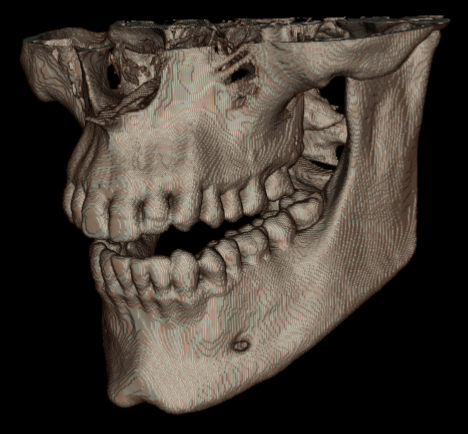
\includegraphics[width=\textwidth]{BSS}
        \caption{Side View of Volume}
    \end{subfigure}
    \hfill
    \begin{subfigure}[b]{0.33\textwidth}
        \centering
        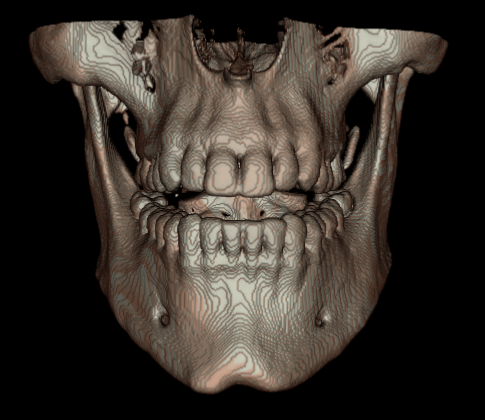
\includegraphics[width=\textwidth]{BSF}
        \caption{Front View of Volume}
    \end{subfigure}
      \hfill
    \begin{subfigure}[b]{0.33\textwidth}
        \centering
        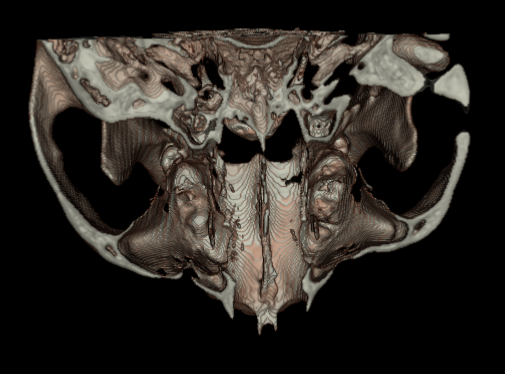
\includegraphics[width=\textwidth]{BST}
        \caption{Top View of Volume}
    \end{subfigure}
    \caption{Volume of Interest Before Segmentation with different Views}
    \label{fig:BS}
\end{figure}


\begin{figure}
    \centering
    \begin{subfigure}[b]{0.33\textwidth}
        \centering
        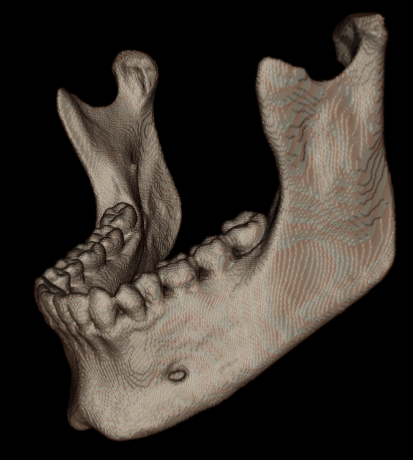
\includegraphics[width=\textwidth]{RCS}
        \caption{Side View of Volume}
    \end{subfigure}
    \hfill
    \begin{subfigure}[b]{0.33\textwidth}
        \centering
        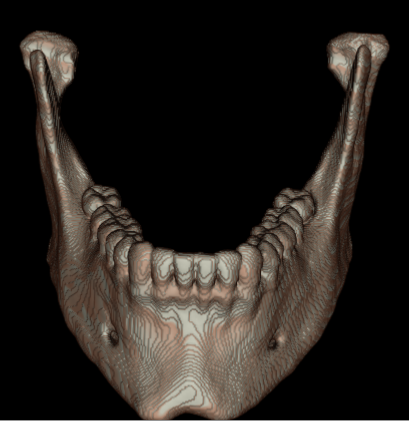
\includegraphics[width=\textwidth]{RCF}
        \caption{Front View of Volume}
    \end{subfigure}
      \hfill
    \begin{subfigure}[b]{0.33\textwidth}
        \centering
        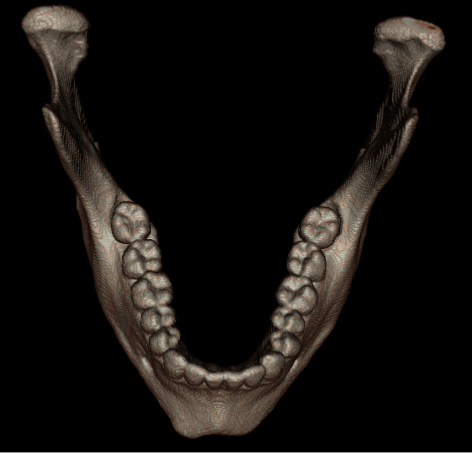
\includegraphics[width=\textwidth]{RCT}
        \caption{Top View of Volume}
    \end{subfigure}
    \caption{Rendering of Volume After Segmentation with different Views using  Ray Casting rendering technique.}
    \label{fig:RC}
\end{figure}

\begin{figure}
    \centering
    \begin{subfigure}[b]{0.33\textwidth}
        \centering
        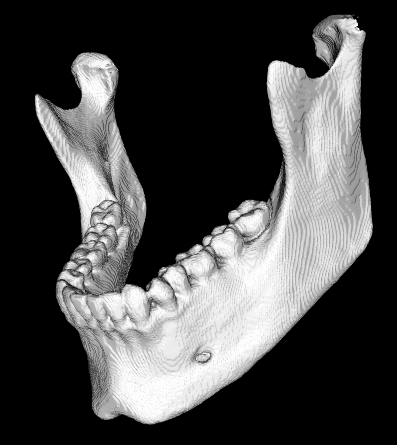
\includegraphics[width=\textwidth]{MCS}
        \caption{Side View of Volume}
    \end{subfigure}
    \hfill
    \begin{subfigure}[b]{0.33\textwidth}
        \centering
        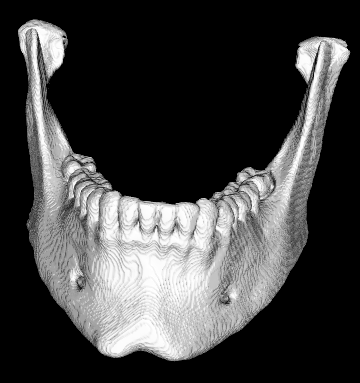
\includegraphics[width=\textwidth]{MCF}
        \caption{Front View of Volume}
    \end{subfigure}
      \hfill
    \begin{subfigure}[b]{0.33\textwidth}
        \centering
        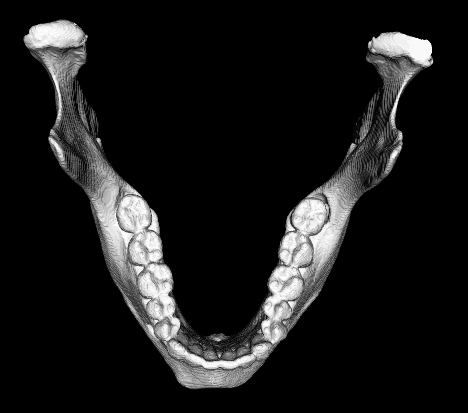
\includegraphics[width=\textwidth]{MCT}
        \caption{Top View of Volume}
    \end{subfigure}
    \caption{Rendering of Volume After Segmentation with different Views using  Marching Cubes rendering technique.}
    \label{fig:MC}
\end{figure}


\begin{figure}
    \centering
    \begin{subfigure}[b]{0.33\textwidth}
        \centering
        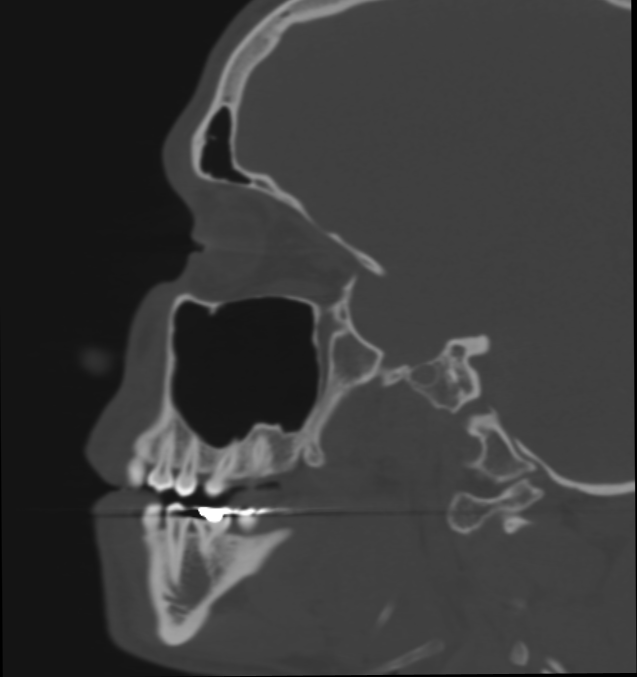
\includegraphics[width=\textwidth]{NSV}
        \caption{Sagittal View}
    \end{subfigure}
    \hfill
    \begin{subfigure}[b]{0.33\textwidth}
        \centering
        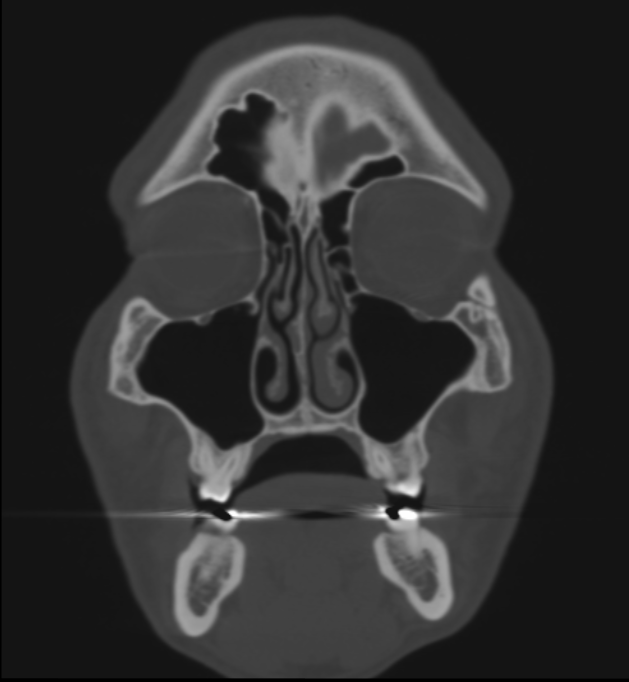
\includegraphics[width=\textwidth]{NFV}
        \caption{Coronal View}
    \end{subfigure}
      \hfill
    \begin{subfigure}[b]{0.33\textwidth}
        \centering
        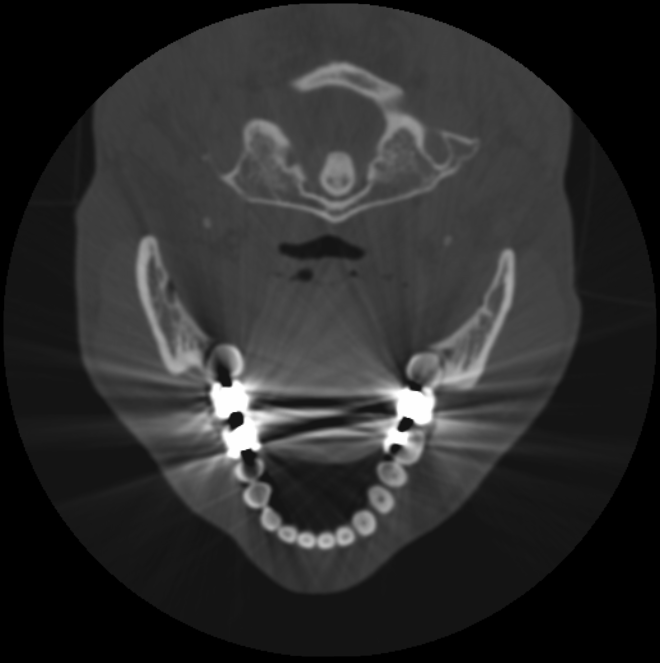
\includegraphics[width=\textwidth]{NTV}
        \caption{Axial View}
    \end{subfigure}
    \caption{The Different projections of case 13 that contains artifacts.}
    \label{fig:NV}
\end{figure}

\begin{figure}
\centering 
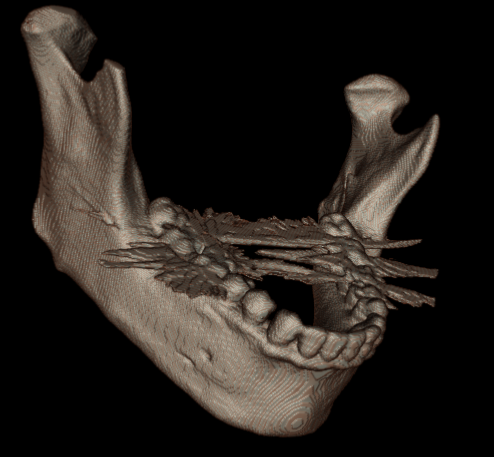
\includegraphics[scale=0.5]{NS}
\caption{The Result of segmentation of case 13 that contains artifacts}
\label{fig:NS}
\end{figure}

\section{Missed Objectives}
\begin{itemize}
\item GUI Design
\end{itemize}

\section{Next Step}
\begin{itemize}
\item Saving the mandible as STL Volume.
\item Code enhancement and memory mangement.
\item Design and implement a simple and effective GUI.
\item Searching about artifacts removal.
\end{itemize}   
%******************************************************************************
% DOCUMENT ENDS HERE 
%******************************************************************************
\end{document}